%!TEX encoding = UTF-8 Unicode
% !TeX spellcheck = en_GB
%%%%%%%%%%%%%%%%%%%%%%%%%%%%%%%%%%%%%%
\chapter{Experimental measurements of the Higgs boson }\label{chap:HiggsConstr}
%%%%%%%%%%%%%%%%%%%%%%%%%%%%%%%%%%%%%%
%In this chapter, I will discuss some of the bounds on the Higgs sector . Starting from an overview of the theoretical constraints on the Higgs potential, like the quantum triviality and unitarity. Then, the state-of-the-art experimental results on Higgs properties and couplings measurements will be discussed. However, despite many of the Higgs boson properties have been measured with good accuracy, there are still difficult observables in the Higgs sector and some open problems. These will be addressed at the end of this chapter.   
%%
The observation of the Higgs boson, then the extensive measurement of its properties and couplings has been on the top of the LHC programme priorities~\cite{ellis2000physics}. In the time this thesis was in the writing, the particle physics community will be celebrating a decade since the Higgs boson's discovery. Looking back 10 years ago, when I have witnessed the discovery of the Higgs boson via news press-conference in summer of 2012, and decided to be a part of this enormous step that humanity has taken, 
I feel astonished by the progress made in understanding this newly discovered particle!  \\ In this chapter, I will start by an overview of the extraordinary LHC and its experiments~in~\autoref{sec:theLHC}. Then, I will review the state-of-the-art status of experimental measurements of the Higgs properties in~\autoref{sec:Higgsprop}, cross-sections  and couplings in ~\autoref{sec:Higgscoupl}, and at the end I will discuss the challenges and outlook for the future runs of the LHC~\autoref{sec:Higgscouplchallenge}, of which the of the rest of this thesis is going to be aim address a small part of them.
\section{Overview of the Large Hadron Collider \label{sec:theLHC}}
\par The Large Hadron Collider~(LHC) is the largest particle accelerator in the CERN accelerators complex, with a circumference of about 26 \si{\kilo\metre},with over 9590 superconducting magnets cooled to 1.9 \si{\kelvin}. It was built as an upgrade to the  Large electron positron collider~(LEP) which ended its operation in the year 2000. The LHC contains four main experiments situated at the four beam collision points and detectors, and these experiments are: ATLAS, CMS, LHCb and ALICE, there also smaller experiments such as LHCf, MilliQan,TOTEM and others. For more details about the LHC cf.~\cite{cernfacts,welt-machine} or see the LHC technical design report~\cite{Bruning:2004ej} for more technical details.\\   The LHC started operation in September of 2008, with low energy proton beams, then gradually increased to an energy of 3.5 \TeV\ per proton to reach a centre of mass energy~$\sqrt{s}$ of 7 \TeV, and data-taking period started from 2011 . By 2012, its energy has increased to $\sqrt{s}= 8\ \TeV$ and operated at this energy for about year and half, then stopping in mid 2013 concluding what is known as \textbf{Run-I}. In 2015, the \textbf{Run-II} started with almost double the energy $\sqrt{s}= 13\ \TeV$, and lasted for ca. 3 years. As this thesis being written, preparations are being made to get \textbf{Run-III} started until 2024. During these runs, heavier nuclei such as $\prescript{207}{}{\mathbf{Pb}}$ and $\prescript{131}{}{\mathbf{Xe}}$ have been collided either with protons or with themselves~\cite{lhckomission}.  \\  From, 2025 and beyond, the \textbf{High-Luminosity} LHC~(HL-LHC) era will commence, see~\autoref{fig:lhcplan}.   Where the LHC will be shutdown for extensive upgrades ~\cite{Apollinari:2015bam} to potentially increase its energy to  $\sqrt{s}= 14\ \TeV$ and higher collision rates hence the term \emph{high luminosity}. Which leads us to an important notion in particle physics phenomenology ~\emph{integrated luminosity}.\\
\par The performance of colliders depends on many factors, but for phenomenological studies, like this thesis, one mainly considers the centre of mass energy $\sqrt{s}$ and the integrated luminosity~$\mathscr{L}$.
This is mainly due to the fact that particle colliders experiments are basically ``counting experiments'', and all of the bounds on physical observables or model parameters are obtained from the number of signal versus background events, and the number of expected events~$N_{expec}$ for a given resonance $R$ and a subsequent decay final state $X$ at any collider experiments is given by
\begin{equation}
	N_{expec} = \sigma(pp\to R) \, \mathcal B(R \to X)\,\mathscr{L}  \, \epsilon_{\mathrm{SEL}}.
\end{equation}
Here $ \epsilon_{\mathrm{SEL}}$ is the selection efficiency, which depends on many factors like the detector geometry and particle identification performance etc. , as well as the signal one searches for, it can be improved by better detected or selection cuts. The production cross-section increases typically with quadratically with $\sqrt {s}$, hence comes the need for higher energies but this can only achieved by building new colliders from scratch. The integrated luminosity can be increased much more easily, by longer running time of the same collider as it is the time integral of the collider's luminosity $L(t)$ over its operation time $T$
\begin{equation}
\mathscr{L} = \int^{T} L(t) .
\end{equation}
Therefore, we see that the integrated luminosity for the LHC experiments will increase over time, when more collisions taking place, as seen in figure~\autoref{fig:lumi} showing the integrated luminosity for ATLAS and CMS experiments. 
\begin{figure}[t!]
	\begin{center}
		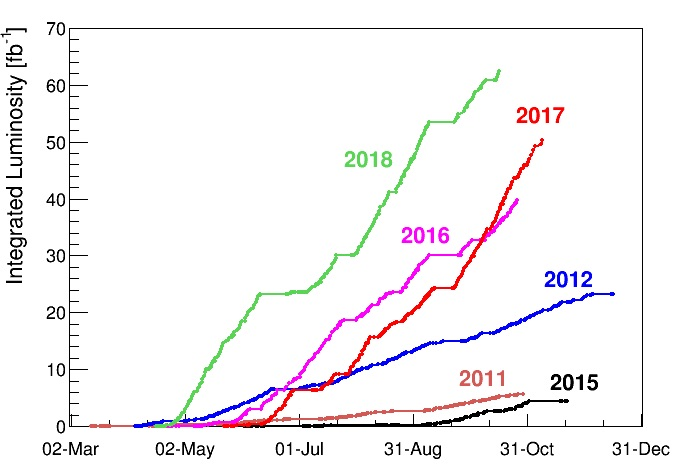
\includegraphics[width=8cm]{figures/lhc_lumi}
		\caption{The integrated luminosity of the CMS and ATLAS experiments combined over the period from 2011-2018, source~\cite{lhcpreformance}.  \label{fig:lumi} }
	\end{center}
\end{figure}
As thee protons travel in the LHC in \textbf{bunches}, and as these bunches cross, protons collide at a certain frequency $f$,  when two bunches with $N_1$ and $N_2$ protons per bunch, respectively. Each bunch will have an effective cross-section~$4 \pi \sigma_i$ corresponding to their physical sizes $\sigma \sim \SI{16}{\micro \meter}$, the luminosity is therefore given -approximately- by 
\begin{equation}
	L = \frac{f N_1 N_2}{4 \pi  \sigma_1 \sigma_2},
\end{equation}
which is for the LHC averages to about $ 10^{34}$ collisions \si{\per \centi\metre\squared \per \second}~\cite{closer,lhcpreformance}.  \\ The total physics-viable $pp$-collisions  integrated luminosity for Run-I was \SI{4.57}{\per \femtobarn} for \SI{7}{\tera\electronvolt} and \SI{20.3}{\per \femtobarn} for \SI{8}{\tera\electronvolt} (ATLAS~\cite{atlaslumi1}) and  \SI{5.55}{\per \femtobarn} at \SI{7}{\tera\electronvolt} and \SI{21.8}{\per \femtobarn} at \SI{8}{\tera\electronvolt} (CMS ~\cite{cmslumi}). As for Run-II the integrated luminosity is \SI{139}{\per \femtobarn} at \SI{13}{\tera\electronvolt } (ATLAS~\cite{atlaslumi2})  and \SI{137}{\per \femtobarn} at \SI{13}{\tera\electronvolt } (CMS ~\cite{cmslumi}). The expected integrated luminosity by the end of Run-III is  \SI{300}{\per \femtobarn}~\cite{Fartoukh:2790409} and \SI{3000}{\per \femtobarn} by the end of the HL-LHC at energy of \SI{14}{\tera\electronvolt }~\cite{Apollinari:2015bam}. 
\begin{sidewaysfigure}[ht]
	\centering
		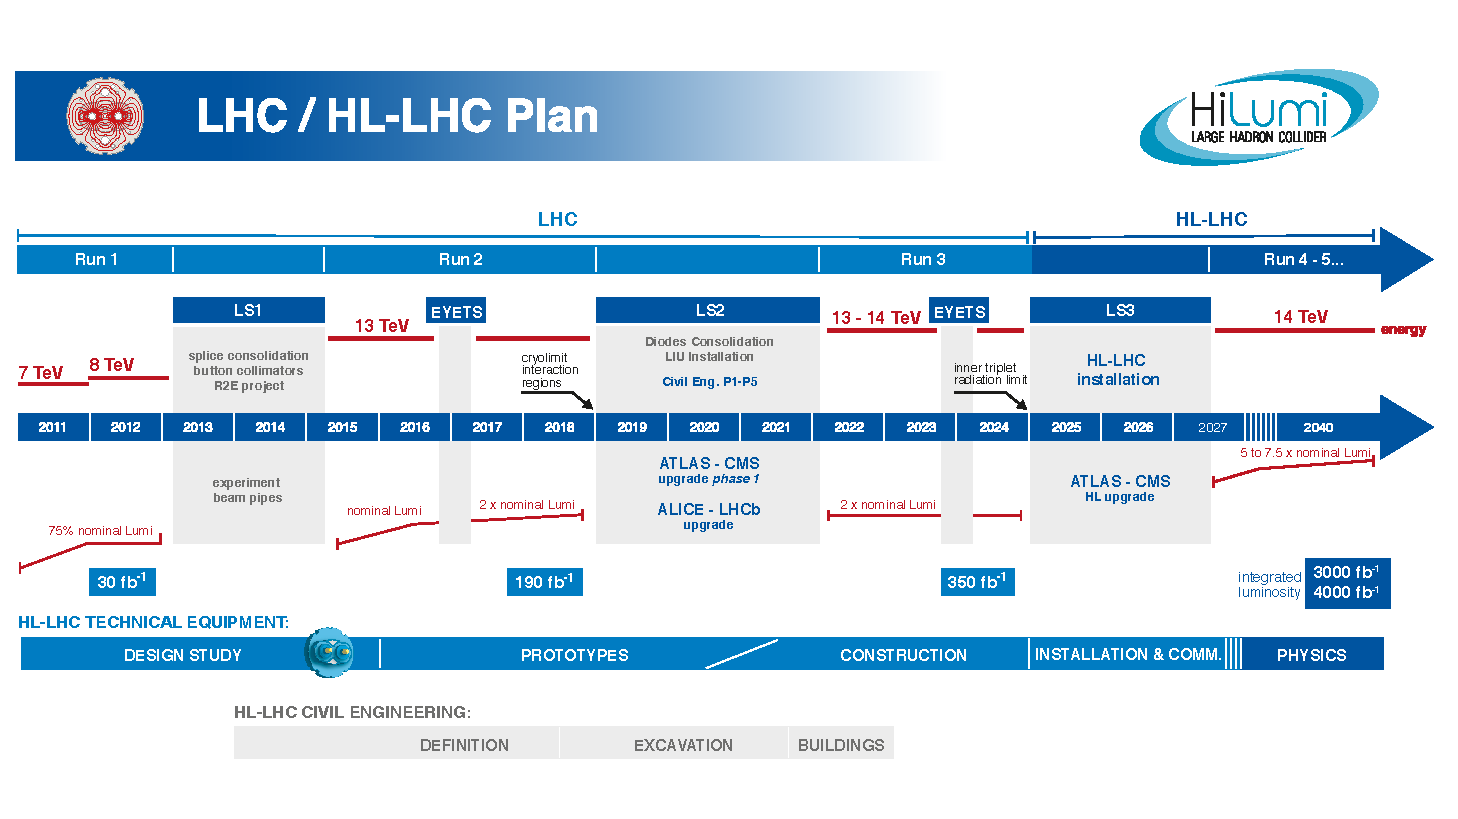
\includegraphics[width=\textwidth]{figures/HL-LHC-plan-2021-1}
	\caption{ A timeline of the LHC operation showing Run-I, Run-II and future planned runs of the LHC, including the HL-LHC, source~~\cite{lhckomission}. 
	}
\label{fig:lhcplan}
\end{sidewaysfigure}
\FloatBarrier
\section{Higgs properties \label{sec:Higgsprop} }
\subsection{Higgs boson mass measurements}
In order to measure the mass of thee Higgs boson with high precision, one need to consider final states that can be reconstructed with high momentum and mass resolution, this is typically achieved when no hadronic constituents in the decays involved, such as  $ h \to \gamma \gamma$ and $ h \to Z Z^*\to 4 \ell$. Reconstructing the invariant mass distributions $m_{\gamma \gamma}$ and $m_{4\ell}$ one observes that the Higgs peak is narrow over a relatively smooth background, see~\autoref{fig:higgs_mass}, which is ideal for the measurement of the Higgs mass. It should be noted that the width of the resonance is due to the detector resolution and does not correspond to the actual Higgs width.\\
\begin{figure}[t!]
	\begin{center}
		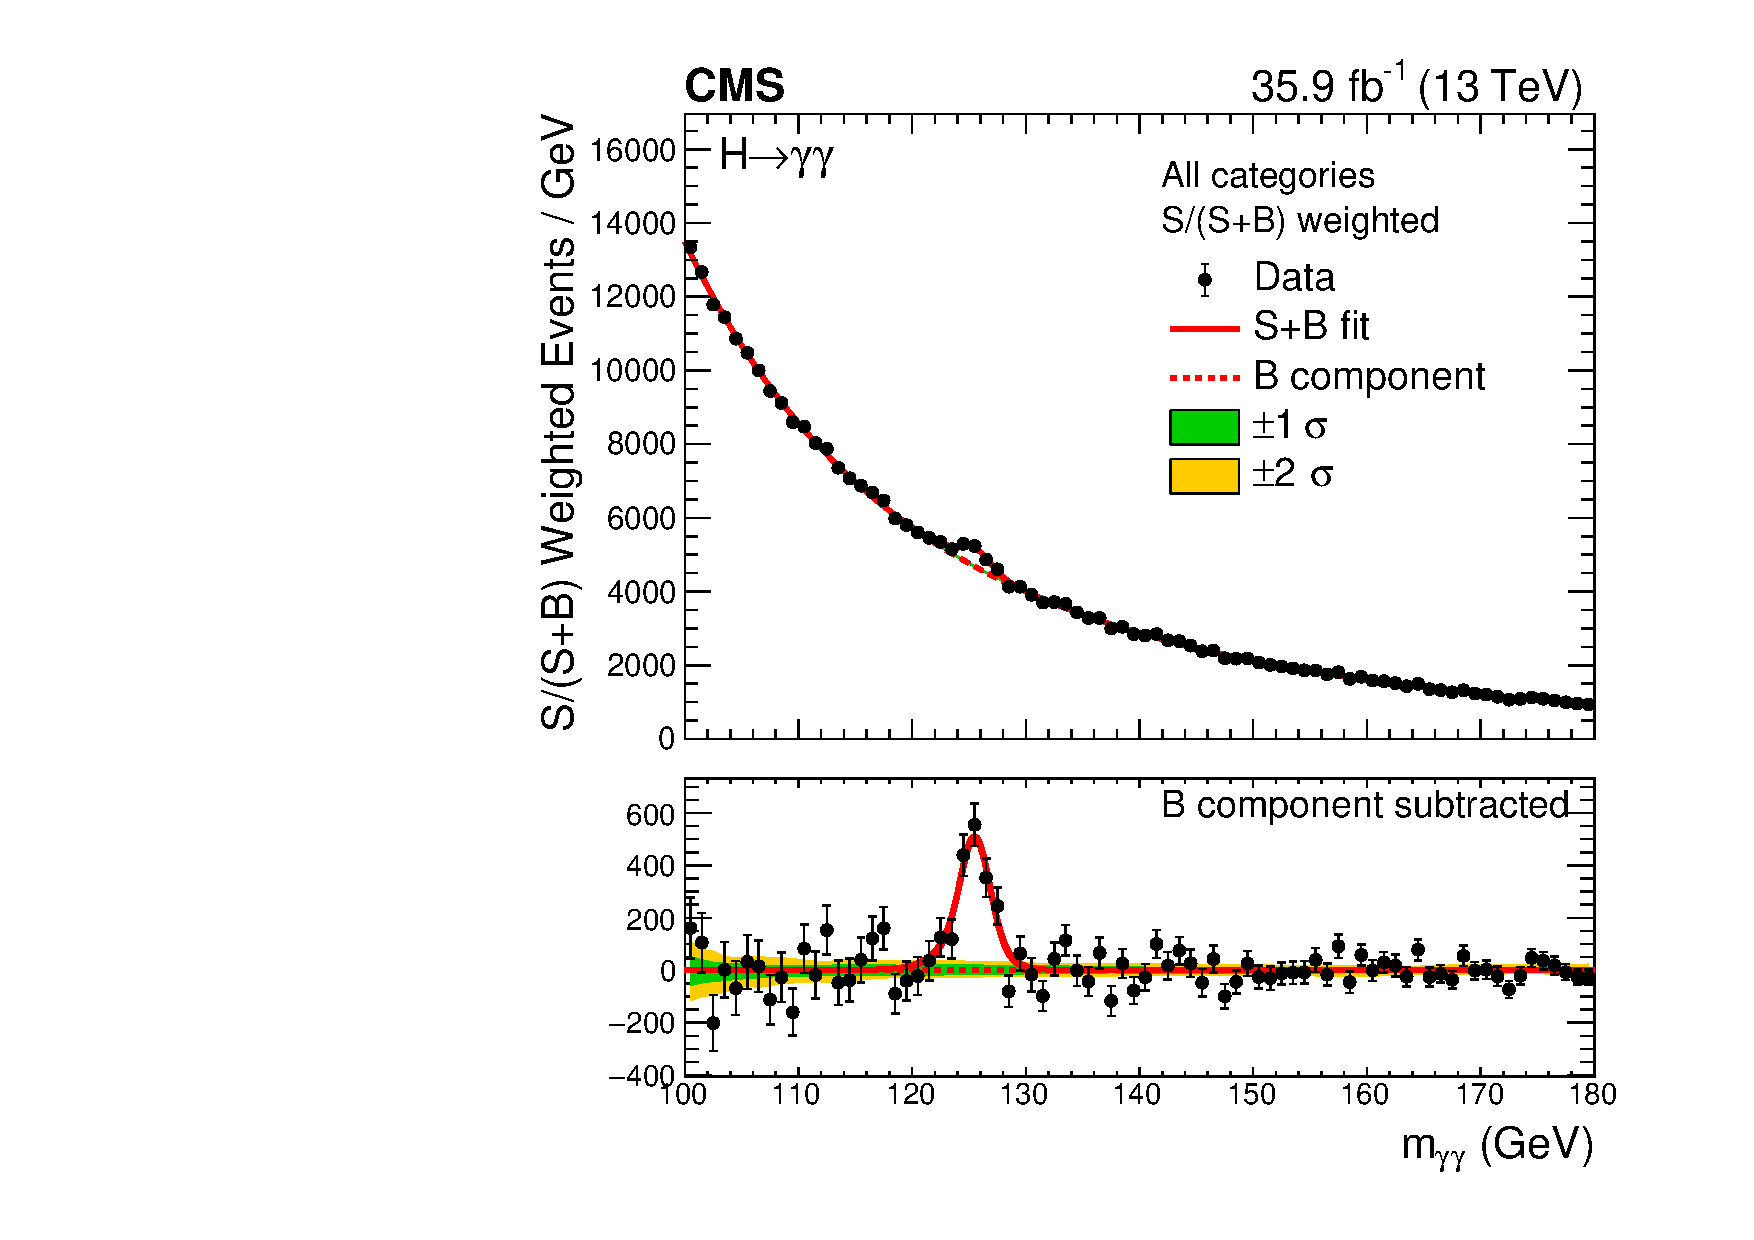
\includegraphics[width=0.45\textwidth]{figures/Higgs_results/CMS-HIG-19-004_Figure_005-b}
		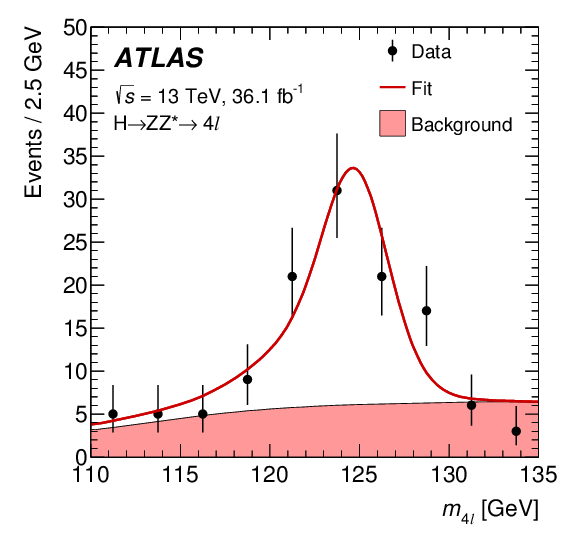
\includegraphics[width=0.45\textwidth]{figures/Higgs_results/dataAll_H4l_m4l_pdf_constrained} 
		\caption{The invariant mass distributions of diphoton~$m_{\gamma \gamma}$ (CMS~\cite{CMS:2020xrn}) and four lepton $m_{4 \ell}$ (ATLAS~\cite{ATLAS:2018tdk}) final states showing a clear peak at the Higgs mass, with smooth background. These final states are ideal for Higgs mass measurements. \label{fig:higgs_mass} }
	\end{center}
\end{figure}
There have been consistent improvements of the Higgs mass measurements since its discovery. In~\autoref{fig:meta_mass} I have preformed a meta analysis on ATLAS and CMS measurements of the Higgs mass in Run-I and Run-II of the LHC for both diphoton and $ZZ^*$ final states based on the data from the studies~\cite{ATLAS:2015yey,ATLAS:2018tdk,CMS:2017dib,CMS:2020xrn} using a random effects model~\cite{aronow_miller_2019}. The pooling of the studies yielded a mass measurement of $ m_h = 125.21 \pm 0.10$, which translates to a $0.11\%$ accuracy, the heterogeneity off the studies was found to be $I^2 =49\%$ ($p=0.05$) . Different measurements combination techniques were used in ~\cite{CMS:2020xrn} and ~\cite{Zyla:2020zbs} yielded different central values but all of the results agree within the uncertainties. 
\begin{figure}[h!]
	\begin{center}
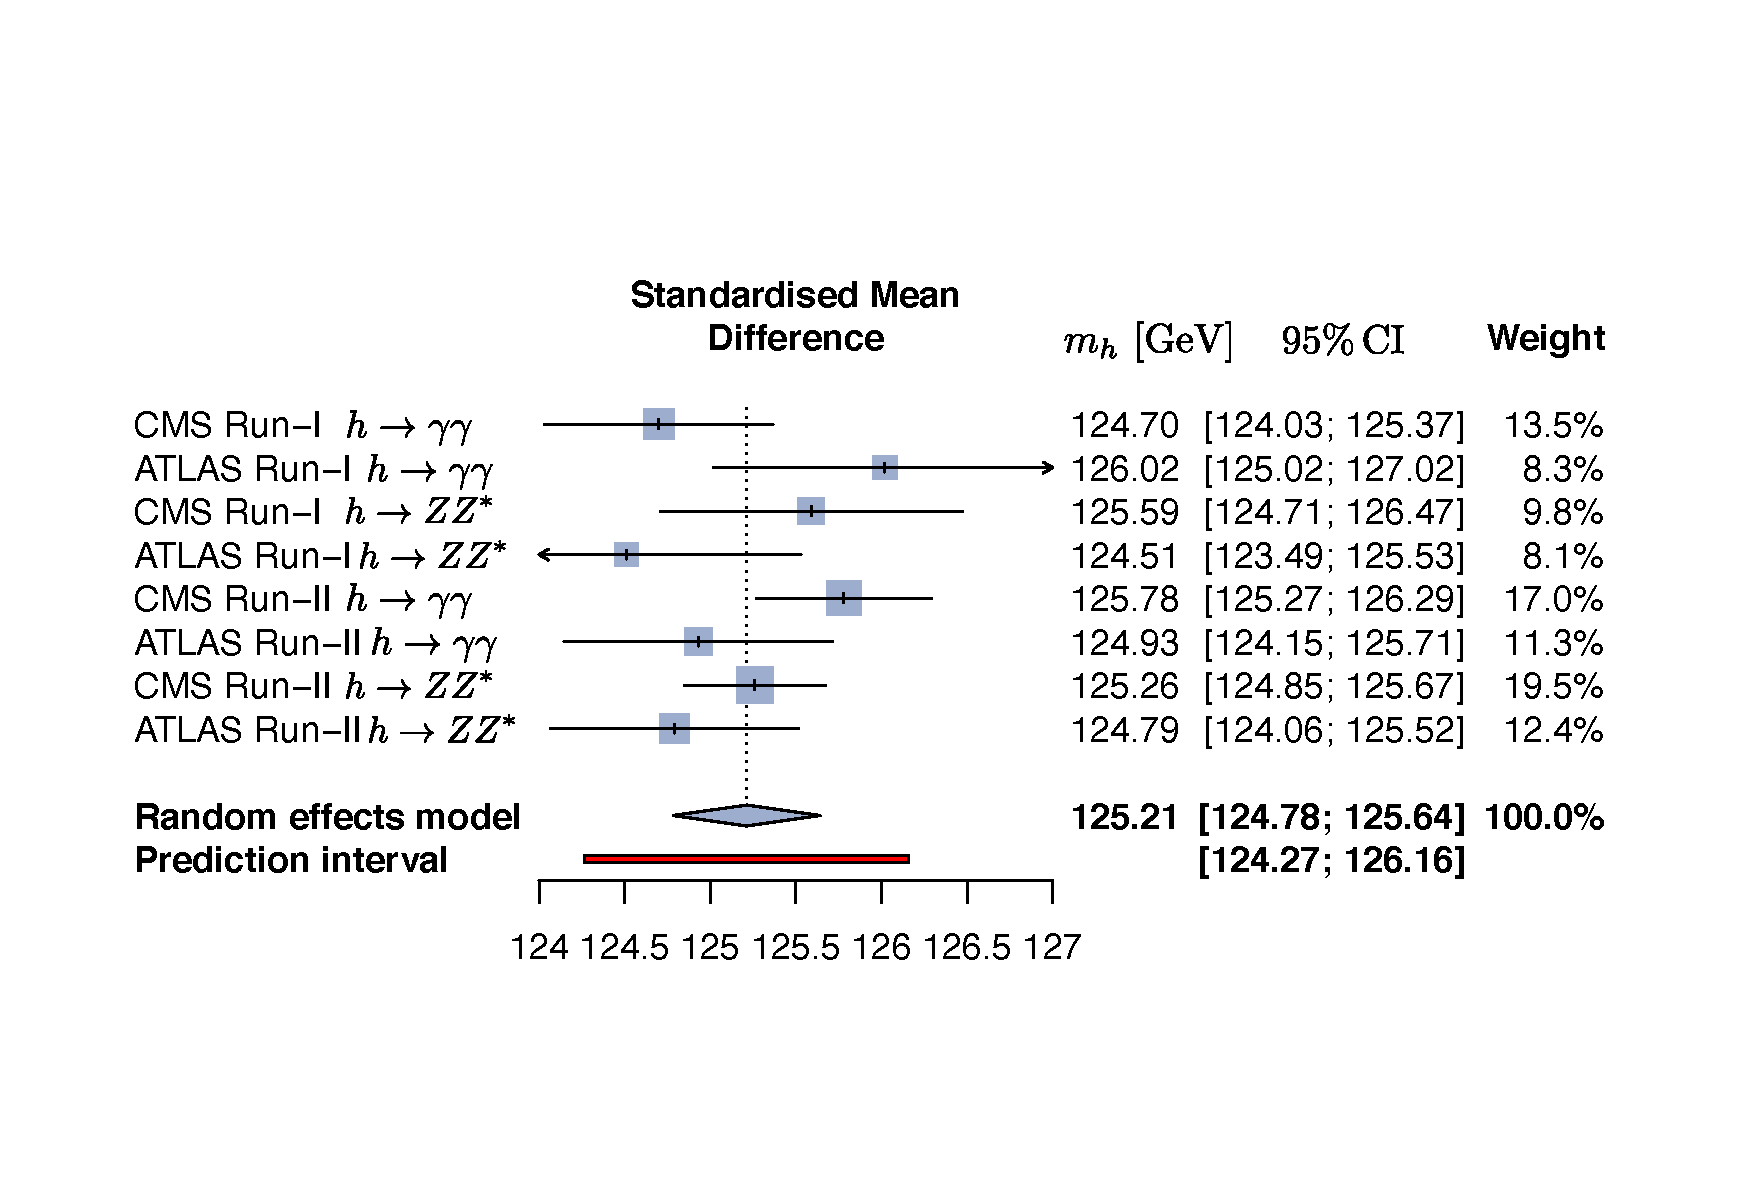
\includegraphics[width=1.\textwidth]{figures/foreest_pllot_higgs_mass}
		\caption{A meta analysis preformed to combine all the measurements of the Higgs mass from Run-I and Run-II, the combined result was obtained from pooling all of the studies using the random effects model method.\label{fig:meta_mass} }
	\end{center}
\end{figure}
\subsection{Higgs full width}
The SM values of the Higgs boson full width is ~$\Gamma_h=4.1$ \GeV\, and it can be accessed in the LHC by looking at the ratio of on-shell versus off-shell Higgs production and decay to the $ZZ^{(*)}$ state, and $ZZ^{(*)}\to 4 \ell, 2 \ell 2 \nu$, namely
\begin{equation}
\frac{\sigma(gg \to h\to Z Z^*)}{\sigma(gg \to h^*\to Z Z)} = \kappa_g^2 \kappa_Z^2 \frac{4 m_Z^2}{m_h \Gamma_h},
\label{widthform}
\end{equation}
where the $\kappa$ here denote the ratio between the measured/ or modified coupling with the Higgs and the SM prediction, i.e.
\begin{equation}
\kappa_X := \frac{g_{XX h}}{g_{XXh}^{\SM}}.
\label{kappa}
\end{equation}
Which is commonly used in reporting experimental constrains/ measurements of the Higgs couplings, as in the next section~\autoref{sec:Higgscoupl}. We shall discuss the $\kappa$ formalism more in~\autoref{chap:HiggsEFT}. \\ We see from~\eqref{widthform} that if one fixes the coupling between the gluons and the $Z$ boson and the Higgs it is possible to access the full width directly.  Unfortunately, it is not possible to directly measure the Higgs full width at the LHC, as this requires full reconstruction of the collision event and study the recoil mass which is only possible at lepton colliders~\cite{DeBlas:2019qco,Banerjee:2021huv}. 
Alas, it is still possible to extract bounds on $\Gamma_h$ using ~\eqref{widthform}. ATLAS used this method to constrain the full width of the Higgs using Run-II data~\cite{ATLAS:2018jym}, while CMS has preformed the same analysis using Run-I and Run-II data combined~\cite{CMS:2019ekd}, the results are 95\% CL bounds of $\Gamma_h$
\begin{align}
\Gamma_h &< \SI{14.4}{\giga\electronvolt} \,\,\,\, (\text{ATLAS}) & \SI{0.08}{\giga\electronvolt} <&\Gamma_h < \SI{9.16}{\giga\electronvolt}  \,\,\,\, (\text{CMS}),
\end{align}
with the combined bound being  $\sim 3 \Gamma_h^{\SM}$. 
\section{Measurements of Higgs rates and couplings \label{sec:Higgscoupl} }

\subsection{Anomalous couplings  }
to measure $HVV$ CMS used the same data for extraction of the $\Gamma_h$ to study this~\cite{CMS:2019ekd}
\begin{figure}[t!]
	\begin{center}
		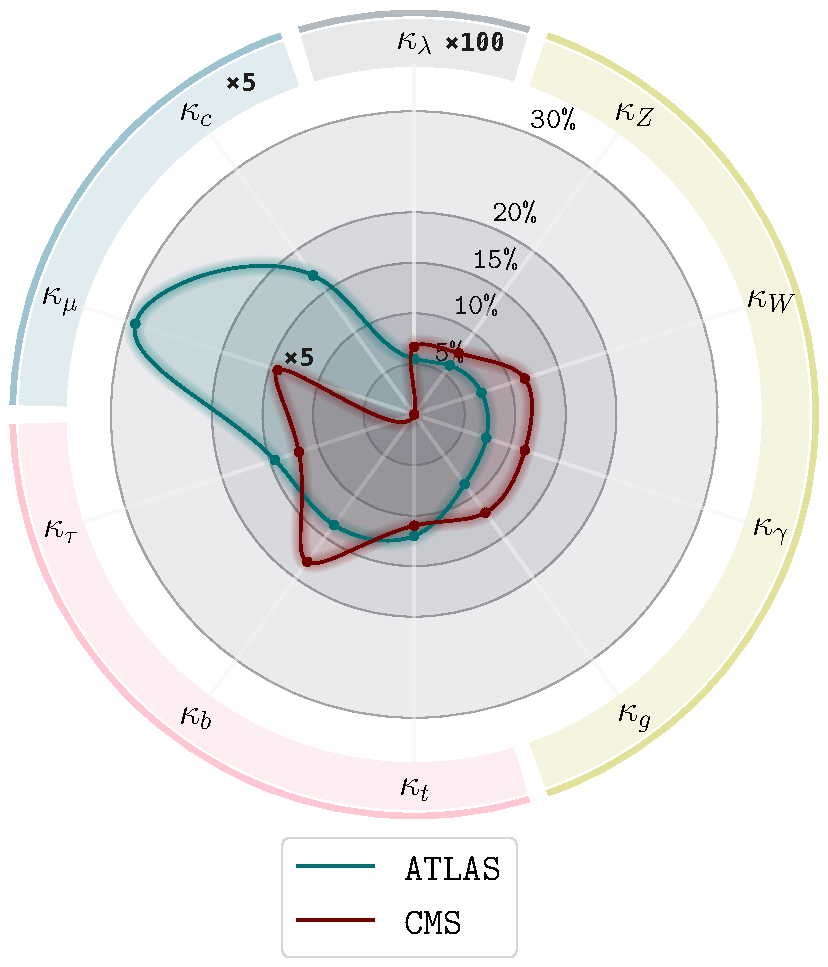
\includegraphics[width=12cm]{figures/Higgs_couplings_poster}
		\caption{ddd  \label{fig:higgs_kappa}}
	\end{center}
\end{figure}
\newpage
\begingroup
\thispagestyle{plain}
\begin{table}[htb!]
\centering
\vspace{-1 cm}
 \footnotesize{ 
	{\renewcommand{\arraystretch}{0.75 }%
\begin{tabular}{clccc}
\toprule
\toprule
\multirow{5}{*}{ {\normalsize Production}}  &\multirow{5}{*}{ {\normalsize Decay}}&\multicolumn{2}{c}{ $\mu_{\mathrm{Exp}} \pm \delta \mu_{\mathrm{Exp}}$  (symmetrised)} &\multirow{5}{*}{ {\normalsize Ref.}} \\
%\cmidrule(r){3-4}
&   & { \bf     \scriptsize           LHC Run-II}&{ \bf  \scriptsize HL-LHC}&   \\
\cmidrule(r){3-4}
&   & { \scriptsize                   CMS $137 \, \mathrm{fb}^{-1} $}&  \multirow{2}{*}{CMS $3 \, \mathrm{ab}^{-1}$}&   \\
&   &  { \CG \scriptsize                   ATLAS $139 \, \mathrm{fb}^{-1} $} & &  \\
\midrule
\midrule
\multirow{ 13}{*}{ \normalsize ggF}         & \multirow{2}{*}{$h\to \gamma  \gamma$} & { \scriptsize                  $0.99 \pm 0.12$}& \multirow{2}{*}{$1.000\pm 0.042$}& \multirow{2}{*}{\cite{ATLAS:2020qdt,CMS:2021kom,CMS-PAS-FTR-18-011}}\\
                                           &                                                          &{ \scriptsize                   \CG $1.030 \pm 0.110$}&& \\ 
                                           \cmidrule(r){2-5}
                                           %%%%%%
                                    &  \mr{$h\to Z Z^*$}          & { \scriptsize                  $0.985 \pm 0.115$}&\multirow{2}{*}{$1.000 \pm 0.040$}&\multirow{7}{*}{\cite{ATLAS:2020qdt,CMS:2020gsy,CMS-PAS-FTR-18-011}}  \\
                                     &                                                      &{ \scriptsize                   \CG $0.945 \pm 0.105$}&& \\
                                     \cmidrule(r){2-4}
                                       %%%%%%
                                    &\mr{ $h\to W W^*$}         & { \scriptsize                  $1.285 \pm 0.195$} &\mr{ $1.000 \pm 0.037$} &\\
                                    & &                                            { \scriptsize                   \CG$1.085 \pm 0.185$} & &\\
                                                                         \cmidrule(r){2-4}
                                     %%%%%%
                                    &\mr{ $h\to \tau^+\tau^- $ }         & { \scriptsize                  $0.385 \pm 0.385$} &\mr{ $1.000 \pm 0.055$} &\\
                                 & &                                            { \scriptsize                   \CG$1.045 \pm 0.575$} & &\\
                                 \cmidrule(r){2-5}
                                 %%%%%%

                                  &\mr{ $h\to  b \bar b$  }      & { \scriptsize                 $2.54 \pm 2.44$} &\mr{ $1.000 \pm 0.247$} &\mr{\cite{CMS:2020gsy,CMS-PAS-FTR-18-011}}\\
                               & &                                            { \scriptsize                   \CG--} & &\\
                                 \cmidrule(r){2-5}
                               %%%%%%  %%%%%%   %%%%%%
                                  &\mr{ $h\to  \mu^+ \mu^-$  }      & { \scriptsize      $0.315 \pm 1.815$} &\mr{ $1.000 \pm 0.138$} &\mr{\cite{CMS:2020gsy,CMS-PAS-FTR-18-011} }\\
& &                                            { \scriptsize                   \CG--} & &\\
%%%%%%  %%%%%%   %%%%%%                               
\midrule
\midrule
%\crowcolor
\multirow{13}{*}{ \normalsize VBF}      
                                     %%%%%%
										&\mr{ $h\to \gamma  \gamma$ }         & { \scriptsize                  $1.175 \pm 0.335$ } &\mr{ $1.000 \pm 0.128$} & \mr{\cite{ATLAS:2020qdt,CMS:2021kom,CMS-PAS-FTR-18-011}}\\
										& &                                           { \scriptsize                   \CG$1.325 \pm 0.245$} & &\\
\cmidrule(r){2-5}
%%%%%%                                   
                                     &\mr{$h\to Z Z^*$ }         & { \scriptsize                  $0.62 \pm 0.41$ } &\mr{ $1.000 \pm 0.134$} & \multirow{7}{*}{\cite{ATLAS:2020qdt,CMS:2020gsy,CMS-PAS-FTR-18-011}}\\
                                    & &                                            { \scriptsize                   \CG$1.295 \pm 0.455$} & &\\
                                                                                             \cmidrule(r){2-4}
%%%%%%

                                   &\mr{$h\to W W^*$}         & { \scriptsize                  $0.65 \pm 0.63$ } &\mr{ $1.000 \pm 0.073$} & \\
                                    & &                                            { \scriptsize                   \CG$0.61 \pm 0.35$} & &\\
 \cmidrule(r){2-4}
%%%%%%0
                                   &\mr{$h\to \tau^+\tau^- $}         & { \scriptsize                  $1.055 \pm 0.295$ } &\mr{ $1.000 \pm 0.044$} & \\
& &                                            { \scriptsize                   \CG$1.17 \pm 0.55$} & &\\
\cmidrule(r){2-5}
%%%%%%0                                    
                                    &\mr{$h\to  b \bar b$}         & { \scriptsize                   -- } &\mr{--} & \mr{\cite{ATLAS:2020qdt} }\\
                                    & &                                            { \scriptsize                   \CG$3.055 \pm 1.645$} & &\\
                                    
                                  \cmidrule(r){2-5}
 %%%%%%  %%%%%%   %%%%%%
 &\mr{ $h\to  \mu^+ \mu^-$  }      & { \scriptsize               $3.325 \pm 8.075$} &\mr{ $1.000 \pm 0.540$} &\mr{ \cite{CMS-PAS-FTR-18-011}}\\
 & &                                            { \scriptsize                   \CG--} & & \\                                   
\midrule
\midrule
\multirow{10}{*}{ \normalsize  $t\bar t h$} 
%%%%%%0                                    
&\mr{ $h\to \gamma  \gamma$}         & { \scriptsize                $1.43 \pm 0.30$ } &\mr{$1.000 \pm 0.094$} & \mr{ \cite{ATLAS:2020qdt,CMS:2021kom,CMS-PAS-FTR-18-011} }\\
& &                                            { \scriptsize                   \CG$0.915 \pm 0.255$} & &\\

\cmidrule(r){2-5}

                                    
%%%%%%0                                    
&\multirow{3}{*} { $h\to V V^*$   }         & { \scriptsize              $0.64 \pm 0.64$({\color{Mahogany}$ZZ^*$}) } &{ \scriptsize   $1.000 \pm 0.246$ ({\color{Mahogany}$ZZ^*$}) } & \multirow{8}{*}{\cite{ATLAS:2020qdt,CMS:2020gsy,CMS-PAS-FTR-18-011}}  \\
& &                                            { \scriptsize                   $0.945\pm 0.465$ ({\color{Mahogany} $W W^*$})} & { \scriptsize   $1.000 \pm 0.097$ ({\color{Mahogany} $W W^*$})} &\\
& &                                            { \scriptsize                   \CG $1.735 \pm 0.545$} & { \scriptsize   --}&\\
\cmidrule(r){2-4}                                    

&\mr{$h\to \tau^+\tau^- $}         & { \scriptsize                $0.845 \pm 0.705$} &\mr{ $1.000 \pm 0.149$} & \\
& &                                            { \scriptsize                   \CG $1.27 \pm 1.0$} & &\\
\cmidrule(r){2-4}                                    

&\mr{ $h\to  b \bar b$  }         & { \scriptsize                 $1.145 \pm 0.315$} &\mr{ $1.000 \pm 0.116$} & \\
& &                                            { \scriptsize                   \CG $0.795 \pm 0.595$} & &\\                                                        
\midrule
\midrule
\multirow{9}{*}{ \normalsize $Vh$}        

                      
&\mr{ $h\to \gamma  \gamma$  }         & { \scriptsize   $0.725 \pm 0.295$ } &{ \scriptsize   $1.000 \pm 0.233$ ({\color{Mahogany}$Zh$}) } & \multirow{2}{*}{ \cite{ATLAS:2020qdt,CMS:2021kom,CMS-PAS-FTR-18-011}  }  \\
& &                                            { \scriptsize                   \CG $1.335 \pm 0.315$} & { \scriptsize   $1.000 \pm 0.139$ ({\color{Mahogany} $W^\pm h$})} &\\
\cmidrule(r){2-5}           
%%%%%%0              
                                    
&\mr{ $h\to Z Z^*$    }         & { \scriptsize   $1.21 \pm 0.85$ } &{ \scriptsize   $1.000 \pm 0.786$ ({\color{Mahogany}$Zh$}) } & \multirow{2}{*}{ \cite{ATLAS:2020qdt,CMS:2020gsy,CMS-PAS-FTR-18-011}  }  \\
& &                                            { \scriptsize                   \CG $1.635 \pm 1.025$} & { \scriptsize   $1.000 \pm 0.478$ ({\color{Mahogany} $W^\pm h$})} &\\
\cmidrule(r){2-5}           
%%%%%%0                                         
                                  
 &\mr{ $h\to W W^*$    }         & { \scriptsize   $1.850\pm 0.438$ } &{ \scriptsize   $1.000 \pm 0.184$ ({\color{Mahogany}$Zh$}) } & \multirow{2}{*}{  \cite{CMS:2021ixs,CMS-PAS-FTR-18-011} }  \\
 & &                                            { \scriptsize                   \CG --} & { \scriptsize   $1.000 \pm 0.138$ ({\color{Mahogany} $W^\pm h$})} &\\
 \cmidrule(r){2-5}           
 %%%%%%0                                                                                                            
 &\mr{$h\to  b \bar b$      }         & { \scriptsize  -- } &{ \scriptsize   $1.000 \pm 0.065$ ({\color{Mahogany}$Zh$}) } & \multirow{2}{*}{  \cite{ATLAS:2020qdt,CMS-PAS-FTR-18-011} }  \\
& &                                            { \scriptsize                   \CG $1.025 \pm 0.175$} & { \scriptsize   $1.000 \pm 0.094$ ({\color{Mahogany} $W^\pm h$})} &\\

%%%%%%0                                        
                                    
\midrule
\midrule
\multirow{2}{*}{ \normalsize $Zh$ { \scriptsize {\color{Mahogany} CMS     }   }}    & $h\to \tau^+\tau^- $ & $1.645 \pm 1.485$&\multirow{5}{*}{--} &\multirow{5}{*}{ \cite{CMS:2020gsy} }  \\
& $h\to  b \bar b$       &$0.94 \pm 0.32$&&\\                         
 \cmidrule(r){2-3}    
\multirow{2}{*}{ \normalsize $W^\pm h${ \scriptsize {\color{Mahogany} CMS     }   }}           & $h\to \tau^+\tau^- $ &$3.08 \pm 1.58$&&\\
& $h\to  b \bar b$      & $1.28 \pm 0.41$&&\\                  
\midrule
\midrule
\end{tabular}
}
}
\caption{The experimental single Higgs production and decay rates measurements from the  complete  data of LHC Run II and projections for the HL-LHC. The uncertainties were symmetrised here. The table is published in~\cite{Alasfar:2022zyr}.  }
\label{table:resHiggsExp}
\end{table} 
\endgroup
\section{Challenges and outlook \label{sec:Higgscouplchallenge} }
%We also provide in this appendix the experimental measurements of the signal strengths at the LHC Run II and the CMS projections for the HL-LHC (scenario S2, see \cite{Cepeda:2019klc}) that we used in the fits in this paper. These inputs are summarised in table~\ref{table:resHiggsExp}.
